\documentclass[../../TAU.tex]{subfiles}
\begin{document}

\chapter{Математическое описание непрерывных систем уравнений} % (fold)

    В ТАУ при анализе и синтезе САУ рассматриваются их {\it математические модели}.

    \defi{\it Математическая модель} (ММ) - уравнения, переходные и временные функции, которые описывают процессы, происходящие в САУ.
    Существует два способа получения ММ: теоретический и экспериментальный.\par
    
    {\it Теоретический метод} заключается в аналитическом исследовании физической сущности процесса с использованием общих законов физики, или процессов с использованием материального и энергетического баланса. Применение чисто теоретического метода представляет большую трудность вследствие сложности явлений, происходящих в процессах, или недостаточной степени изученности их.
    
    {\it Экспериментальный метод} математического описания заклю­чается в обработке экспериментальных данных, полученных непо­средственно на действующих объектах производства, или на полу­промышленной лабораторной машине, или физической модели про­цесса — стенде.\par
    Наиболее эффективным методом получения математической модели является сочетание {\itтеоретического} и {\it экспериментального} ме­тодов. При этом на долю теоретического метода приходится анализ в основном структурных свойств объекта и продуктов и получение общего вида уравнений, а на долю экспериментального — количе­ственный анализ и проверка теоретических выводов.\par
    При построении ММ неизбежно возникают противоречивые требования: достаточная точность модели и доступность, или простота, анализа модели. Чем выше точность модели, тем она сложнее; чем проще исследовать ММ, тем она проще. Цель, которую ставит перед собой разработчик или исследователь, разрешает данное противоречие. 




\section{Уравнения динамики и статистики} % (fold)

    Любой элемент (часть) САУ осуществляет преобразование входа 
    $g$ (или $u$) в выход $y$:
    
    \begin{equation}
        y(t) = A g(t),
    \end{equation}
    
    где $A$ --- оператор САУ. В этом курсе мы будем рассматривать только оператор $A$, описываемый обыкновенными дифференциальными уравнениями (ОДУ). Введем два вида уравнений, рассматриваемых в ТАУ.

    \defi{\it Уравнение статистики} - уравнение, описывающее статический (установившийся) режим.
    
    \defi {\it Уравнение динамики} - уравнение, описывающее процесс в звене при произвольных входных воздействиях.

    Пусть дано ОДУ некоторого ОУ вида
    
    \begin{equation}\label{EQ_DYNAMIC}
        F(y,\dot y, \ddot y, u, \dot u, v) = 0,
    \end{equation}
    
    где $F$ --- функция нескольких переменных, $y$ и $u$ --- выход и управление, $v$ --- возмущение.

    Пусть при $u=u^0$ и $v=v^0$ со временем выход $y$ принимает постоянное значение: $y=y^0$. Тогда уравнение 
    \eref{EQ_DYNAMIC} 
    примет вид
    
    \begin{equation}\label{EQ_STATIC}
        F^0=F(y^0, 0, 0, u^0, 0, v^0) = 0.
    \end{equation}
    
    Уравнение 
    \eref{EQ_STATIC} 
    называется уравнением статики, уравнение 
    \eref{EQ_DYNAMIC} 
    называют уравнением динамики.

\subsection{Звено САУ} % (fold)

    \defi{\it Звеном} называют ММ либо части САУ, либо САУ целиком. Понятие звена удобно использовать для представления САУ в виде соединения нескольких звеньев, т.е. более простых ММ.

    Одно из самых простых звеньев - это усилитель, П[ропорциональное]-звено. Его уравнение можно записать в виде
    
    \begin{equation}
        y = ku.
    \end{equation}
    
    Уравнение динамики здесь совпадает с уравнением статики (точнее, динамики просто нет). Такого рода преобразования часто обозначают графически в виде блока.

    \begin{figure}[h]
        \centering
        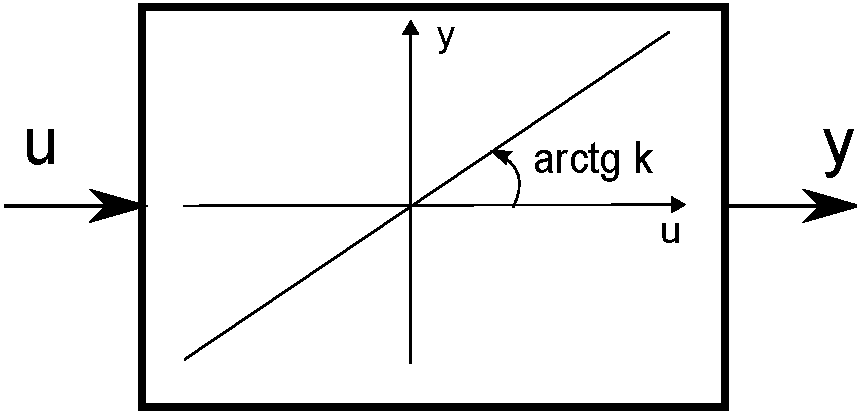
\includegraphics[width=8cm]{block_gain.pdf}
        \caption{Статическая характеристика П-звена}
        \centering
    \end{figure}


    % subsection звено_сау (end)

\subsection{Линеаризация} % (fold)

    Назначение САУ - это поддержание определенного заданного режима. Поэтому параметры, описывающие САУ, не должны сильно отличаться от заданного режима. Эта простая идея обычно позволяет проводить операцию линеаризации.

    \defi{\it Линеаризация} - построение приближенной линейной модели на основе более реалистичной нелинейной модели.

    Рассмотрим пример для уравнения 
    \eref{EQ_DYNAMIC}.

    Пусть заданный режим имеет вид
    \begin{equation}
        y = y^0, \dot y = \ddot y = 0, u=u^0, \dot u = 0, v=v^0.
    \end{equation}
    
    Тогда реальные параметры САУ можно записать в отклонениях как
    
    \begin{equation}
        y = y^0+\Delta y,\;\dot y = \dot{\Delta y},\;\ddot y = \ddot{\Delta y},\; u = u^0 + \Delta u,\; \dot u = \dot{\Delta u},\;v = v^0 + \Delta v,
    \end{equation}
    
    где переменные со знаком $\Delta$ достаточно малы.

    Тогда для функции 
    
    $F(y,\dot y, \ddot y, u, \dot u, v)$ 

    воспользуемся разложением в ряд Тейлора в точке 

    $(y^0, 0,0, u^0, 0, v^0)$:
    
    \begin{multline}
        F(y,\dot y, \ddot y, u, \dot u, v) = F^0 + \frac{\partial F}{\partial y} \Delta y +\frac{\partial F}{\partial \dot y} \dot{\Delta y}+ \frac{\partial F}{\partial \ddot y} \ddot{\Delta y} +\\  + \frac{\partial F}{\partial u} \Delta u + \frac{\partial F}{\partial \dot u } \dot{\Delta u} + \frac{\partial F}{\partial v} \Delta v + \ldots,
    \end{multline}

    где $F^0= 0$, многоточием обозначены члены с более высоким порядком малости.

    Отсюда получают линеаризацию уравнения 
    \eref{EQ_DYNAMIC} 
    вида

    \begin{equation}\label{EQ_LINEAR}
        a_2\ddot{\Delta y} + a_1 \dot{\Delta y} + a_0 \Delta y - b_1\dot{\Delta u} - b_0\Delta u - c_0 \Delta v = 0,
    \end{equation}

    где 
    $a_0 = \frac{\partial F}{\partial y}$, 
    $a_1 = \frac{\partial F}{\partial \dot y}$, $a_2 = \frac{\partial F}{\partial \ddot y}$, 
    $b_0 = -\frac{\partial F}{\partial u}$, 
    $b_1 = -\frac{\partial F}{\partial \dot u }$ и 
    $c_0 = -\frac{\partial F}{\partial v}$.

    Введем оператор дифференцирования: 
    $s = \frac{d}{dt}$.

    Тогда уравнение 
    \eref{EQ_LINEAR}
     примет вид (знаки $\Delta$ опущены)
    
    \begin{equation}
        a_2 s^2 y + a_1 s y + a_0 y = b_1 s u + b_0 u + c_0 v,
    \end{equation}
    
    что эквивалентно
    
    \begin{equation}
        Q(s) y = R_1(s)u + R_2(s)v,
    \end{equation}
    
    где 
    $Q(s) = a_2s^2 + a_1 s + a_0$ 
    называют {\it собственным оператором}, а 
    $R_1(s) = b_1s+b_0$ и 
    $R_2(s) = c_0$
     --- {\it операторами воздействия}.

    \defi{\it Собственный оператор} - дифференциальный оператор $Q(s)$ при выходной величине.

    \defi{\it Оператор воздействия} - дифференциальный оператор $R(s)$ при входной величине.


    % subsection линеаризация (end)

    % section уравнения_динамики_и_статистики (end)

\section{Преобразование Лапласа} % (fold)

    Для исследования и описания ОДУ часто используют преобразование Лапласа, так как оно сводит решение дифференциальных уравнений к алгебраическим операциям.

    \defi{\it Преобразованием Лапласа} называют отображение 
    $\LAP{\cdot}$ 
    функции 
    $x(t), t\in\BF{R}$
     в функцию 
    $X(s), s\in\BF{C}$
    , осуществляемое по правилу
    
    \begin{equation}
        X(s) = \LAP{x(t)} \stackrel{def}{=} \int\limits_0^\infty e^{-st} x(t) dt,
    \end{equation}
    
    где $x(t)$ --- исходная функция, $X(s)$ --- изображение по Лапласу, $s$~---~переменная преобразования Лапласа.


    Условия, при которых преобразование существует для $x(t)$:
    
    \begin{enumerate}
        \item $x(t)$ --- интегрируемая на любом конечном интервале функция;
        \item $x(t)\equiv0$ при $t < 0$;
        \item $\exists c, M > 0: |x(t)| < M e^{ct}, \forall t \ge 0$.
    \end{enumerate}

    Если $x(t)$ удовлетворяет всем вышеперечисленным свойствам, то её называют функцией-оригиналом.

\subsection{Обратное преобразование Лапласа} % (fold)

    Соотношение, определяющее по известному изображению его оригинал, называют {\it обратным преобразованием Лапласа}. 

    \begin{equation}
        x(t) = \INVLAP{X(s)} = \frac{1}{2\pi j} \int\limits_{\sigma-j\infty}^{\sigma + j\infty} X(s)e^{st} ds,
    \end{equation}
    
    где интегрирование ведется вдоль любой прямой 
    $\RE{s} = \sigma > c$, 
    где $с$ --- константа из условий существования преобразования Лапласа для $x(t)$.

% subsection обратное_преобразование_лапласа (end)

\subsection{Свойства преобразования Лапласа и примеры} % (fold)

    Пусть 
    $X(s) = \LAP{x(t)}$ и 
    $Y(s) = \LAP{y(t)}$.
    
    \begin{enumerate}
        \item Линейность. $\LAP{\alpha x(t) + \beta y(t)} = \alpha X(s) + \beta Y(s);$
        
        \item Дифференцирование оригинала. \\
            Если производная 
            $\dot x(t)$ 
            является функцией-оригиналом, то 
            $\LAP{\dot x(t)} = sX(s) - x(0);$
        
        \item Интегрирование оригинала.
            \begin{equation}
                \LAP{\int\limits_0^tx(\tau)d\tau} = \frac{X(s)}{s};
            \end{equation}
        
        \item Теорема запаздывания. Для любого $\tau>0$:
            \begin{equation}
                \LAP{x(t-\tau)} = e^{-\tau s}X(s);
            \end{equation}
        
        \item  Теорема о свертке (или об умножении изображений).\\
            Если $x(t)$ и $y(t)$ - оригиналы изображений, а $X(t)$ и $Y(t)$ - их изображения, то
            
            \begin{equation}
                X(s)\cdot Y(s) = \LAP{\int\limits_0^tx(\tau)y(t-\tau)d\tau} = \LAP{\int\limits_0^ty(\tau)x(t-\tau)d\tau};
            \end{equation}
            
            Интеграл в правой части называют {\it сверткой функций} $x_1(t)$ и $x_2(t)$, его обозначают $x_1(t) * x_2(t)$:
            
            \begin{equation}
                x_1(t)*x_2(t) = \LAP{\int\limits_0^t x_1(\tau) x_2(t-\tau) d{\tau}} = \LAP{\int\limits_0^t x_2(\tau) x_1(t-\tau)d\tau}.
            \end{equation}
            
            Поэтому 
            
            \begin{equation}
                X_1(s) * X_2(s) = L\{x_1(t) * x_2(t)\}
            \end{equation}

        \item Теорема о предельных значениях.
            \begin{enumerate}[label*={\arabic*}]
                \item 
                    $x(0) = \LAP{\lim\limits_{s\rightarrow\infty}sX(s)}$;
                
                \item Если существует 
                    $x(\infty) = \lim\limits_{t\rightarrow\infty} x(t)$, тогда 
                    $x(\infty) = \lim\limits_{s\rightarrow0} sX(s)$.
            \end{enumerate}
        
        \item Теорема разложения. \\
            Если изображение по Лапласу есть дробно-рациональная функция, т.е. 
            $X(s) = \frac{B(s)}{A(s)}$, где 
            $A(s)$ и $B(s)$ --- полиномы от $s$ и 
            $\deg A(s) > \deg B(s)$. 
            Тогда
            
            \begin{equation}
                x(t) = \sum_{k=1}^q\frac{1}{(n_k-1)!}\lim\limits_{s\rightarrow s_k} \frac{d^{n_k-1}}{d s^{n_k-1}} (X(s)(s-s_k)^{n_k}e^{ts}),
            \end{equation}
            
            где $s_k$ --- корни уравнения 
            $A(s)=0$, $n_k$ --- кратность $k$-го корня, $q$ --- количество различных корней.
            Когда $q=n$ (все корни простые), тогда
        
            \begin{equation}\label{eq:razl}
                x(t) = \sum^{n}_{k=1}\frac{B(s_k)}{A'(s_k)} e^{s_kt}.
            \end{equation}

    \end{enumerate}

    \examp Определить функцию $x(t)$, изображение которой имеет вид 
    $
        X(s) = \frac{1}{s (s+1)}.
    $\\
    {\bf Решение}\par
    В данном случае

    \begin{equation}
        B(s) = 1,\ A(s) = s (s+1),\ A'(s) = 2 s + 1.
    \end{equation}

    Полюсами функции $X(s)$ являются $s_1 = 0$, $s_2 = -1$, и они являются простыми. Поэтому, согласно формуле \eref{eq:razl} $x(t)=1-e^{-t}$
    
    \begin{table}
        \begin{center}
            \begin{tabular}{|c|c|c|}
            \hline 
            № & Оригинал $x(t)$ & Изображение $X(s)$\\ \hline
            1 & $\delta(t)$ & $1$ \\ \hline
            2 & $1(t)$ & $\frac{1}{s}$ \\ \hline
            3 & $1(t-\tau)$ & $\frac{1}{s} e^{-\tau s}$ \\ \hline
            4 & $t$ & $\frac{1}{s^2}$ \\ \hline
            5 & $t^n$ & $\frac{n!}{s^{n+1}}$ \\ \hline
            6 & $e^{-\alpha t}$ & $\frac{1}{s+\alpha}$ \\ \hline
            7 & $t e^{-\alpha t}$ & $\frac{1}{(s+\alpha)^2}$ \\ \hline
            8 & $t^n e^{-\alpha t}$ & $\frac{n!}{(s+\alpha)^{n+1}}$ \\ \hline
            9 & $\sin{\omega t}$ & $\frac{\omega}{s^2 + \omega^2}$ \\ \hline
            10 & $\cos{\omega t}$ & $\frac{s}{s^2+\omega^2}$ \\ \hline
            11 & $e^{-\alpha t} \sin{\omega t}$ & $\frac{\omega}{(s+\alpha)^2+\omega^2}$ \\ \hline
            12 & $e^{-\alpha t} \cos{\omega t}$ & $\frac{s+\alpha}{(s+\alpha)^2+\omega^2}$ \\ \hline
            \end{tabular}
            \caption{Изображения Лапласа для часто используемых функций}
        \end{center}
    \end{table}

    % subsection свойства_преобразования_лапласа_и_примеры (end)



\subsection{Передаточная функция в изображениях Лапласа} % (fold)

    Рассмотрим линейное уравнение с постоянными коэффициентами вида

    \begin{equation}\label{EQ_ODU}
    y^{(n)} + a_{n-1}y^{(n-1)} + \ldots + a_1 \dot y + a_0y = b_m u^{(m)} + \ldots + b_1 \dot u + b_0 u,
    \end{equation}

    при нулевых начальных условиях, т.е. 
    $y^{(n-1)} (0) = \ldots = \dot y(0) = y(0) = 0, u^{(m-1)} (0) = \ldots = \dot u(0) = u(0) = 0$
    Применяя к обеим частям равенства преобразование Лапласа, получим

    \begin{equation}\label{EQ_W}
    \left(s^n + \sum_{i=0}^{n-1}a_is^i\right) Y(s) = \left(\sum_{i=0}^{m}b_is^i\right) U(s),
    \end{equation}

    где $Y(s) = \LAP{y(t)}$, $U(s) = \LAP{u(t)}$. Разделив уравнение \eref{EQ_W} на полином в левой части, получим

    \begin{equation}  
        Y(s) = W(s)U(s),
    \end{equation}

    где 
    $W(s) = \frac{\beta(s)}{\alpha(s)}$, 
    $\alpha(s) = s^n + \sum_{i=0}^{n-1}a_is^i$ и 
    $\beta(s) = \sum_{i=0}^{m}b_is^i$.

    \defi{\it Передаточной функцией системы \eref{EQ_ODU} в изображениях Лапласа} называется отношение преобразований Лапласа входа и выхода системы при нулевых начальных условиях, причем отношение имеет наименьший порядок.

    Для системы, описываемой уравнением \eref{EQ_ODU}, передаточной функцией является дробно-рациональная функция $W(s)$, в которой были проведены сокращения общих множителей.

    \examp Дана система
    
    $$
        \ddot y - 2\dot y + y = \dot u - u.
    $$
    Найти передаточную функцию $W(s)$.

% subsection передаточная_функция_в_изображениях_лапласа (end)

\subsection{Передаточная функция в операторной форме} % (fold)

    Из записи уравнения \eref{EQ_ODU} в операторной форме вида
    
    \begin{equation}\label{EQ_ODU_SYM_1}
        A(s)y = B(s)u,
    \end{equation}
    
    где 
    $A(s) = s^n + \sum_{i=0}^{n-1}a_is^i$ и 
    $B(s) = \sum_{i=0}^{m}b_is^i$ --- ``составные'' операторы дифференцирования.

    Формально разделив \eref{EQ_ODU_SYM_1} на $A(s)$, получим
    
    \begin{equation}
        y(t) = W(s)u(t),
    \end{equation}
    
    где 
    $W(s) = \frac{B(s)}{A(s)}$ --- передаточная функция (ПФ) системы \eref{EQ_ODU} в операторной форме.

    Заметим, что ПФ в операторной форме и в изображениях Лапласа совпадают, если полиномы $A(s)$ и $B(s)$ не имеют общих корней. Однако ПФ в изображениях Лапласа всегда можно получить из ПФ в операторной форме, проведя сокращения числителя и знаменателя. Получить из ПФ в изображениях Лапласа ПФ в операторной форме не всегда возможно.

    \examp Определить передаточные функции звеньев, описываемых уравнениями:
    
    \begin{tasks}(2)
        \task $\dot y + y = u$
        \task $\ddot y - y = \dot u - u$
    \end{tasks}
    {\bf Решение.}
    В символической форме эти уравнения записываются в виде:

    \begin{tasks}(2)
        \task $(p+1) y = u$
        \task $(p^2-1) y = (p-1) u$
    \end{tasks}

    Их передаточные функции в операторной форме соответственно равны

    $$
        W_1(p)=\frac{1}{s+1}, \ W_2(p)= \frac{p-1}{p^2-1}
    $$

    Передаточные функции в изображениях Лапласа имеют вид

    $$
        \left.W_1(s)=W_1(p)\right\vert_{p=s} = \frac{1}{s+1}, \ 
        \left.W_2(s)=W_2(p)\right\vert_{p=s} = \frac{s-1}{s^2-1} = \frac{1}{s+1}.
    $$
% subsection передаточная_функция_в_операторной_форме (end)

\subsection{Временные функции: переходная и весовая функции} % (fold)

    Кроме дифференциальных уравнений и передаточных функций при описании и исследовании линейных систем используют переходные и импульсные переходные функции и их графики - временные характеристики.

    \defi{\it Переходная функция} $h(t)$  - функция, описывающая реакцию системы (звена) на единичное ступенчатое воздействие при нулевых начальных условиях. 
    График переходной функции - кривую зависимости $h(t)$ от времени $t$ - называют {\it переходной} или {\it разгонной характеристикой}.

    \defi{\it Импульсная переходная (весовая)} функция $w(t)$ - функция, описывающая реакцию системы (звена) на единичное импульсное воздействие ($\sigma(t)$) при нулевых начальных условиях.\\ 
    График импульсной переходной функции - кривую зависимости функций w(t) от времени t - называют {\it импульсной переходной характеристикой}.
    Данные функции связаны соотношением - $w(t) = \frac{dh(t)}{dt}$.


% subsection временные_функции (end)

\subsection{ВФ и ПФ в изображениях Лапласа } % (fold)

    По определению ПФ имеем
    
    $$
        Y(s) = W(s)U(s).
    $$

    По определению переходной функции вход имеет вид 
    $u(t) = \IT{X}(t)$ 
    (а~$h(t) = y(t)$), а значит 
    $U(s) = \LAP{u(t)} = \frac{1}{s}$, поэтому
    
    $$
        Y(s) = \frac{W(s)}{s},
    $$
    
    откуда с помощью обратного преобразования Лапласа получаем 
    $h(t) = \INVLAP{\frac{W(s)}{s}}$.

    Аналогично для весовой функции: 
    $u(t) = \delta(t)$ 
    (a $\omega(t) = y(t)$), тогда $U(s)=1$. Получим, что
    
    $$
        Y(s) = W(s),
    $$
    
    откуда 
    $\omega(t) = \INVLAP{W(s)}$.

    Таким образом, имея хотя бы одну из функций ($h(t), \omega(t)$ или $W(s)$), можно восстановить оставшиеся.

% subsection ВФ и ПФ в изображениях Лапласа  (end)

% section преобразование_лапласа (end)

\section{Частотные функции} % (fold)

% section частотные_функции (end)

\section{Основные типы элементарных звеньев} % (fold)


\subsection{Пропорциональное звено} % (fold)

% subsection пропорциональное_звено (end)

\subsection{Дифференциальное звено} % (fold)

% subsection дифференциальное_звено (end)

\subsection{Интегрирующее звено} % (fold)

% subsection интегрирующее_звено (end)

\subsection{Апериодическое звено} % (fold)

% subsection апериодическое_звено (end)

\subsection{Колебательное звено} % (fold)

% subsection колебательное_звено (end)

\subsection{Звено чистого запаздывания} % (fold)

% subsection звено_чистого_запаздывания (end)

% section основные_типы_элементарных_звеньев (end)

%chapter математическое_описание_непрерывных_систем_уравнений (end)
\end{document}